%%%%%%%%%%%%%%%%%%%%%%%%%%%%%%%%%%%%%%%%%%%%%%%%%%%%%%%%%%%%%%%%%%
%%%%%%%% ICML 2013 EXAMPLE LATEX SUBMISSION FILE %%%%%%%%%%%%%%%%%
%%%%%%%%%%%%%%%%%%%%%%%%%%%%%%%%%%%%%%%%%%%%%%%%%%%%%%%%%%%%%%%%%%

% Use the following line _only_ if you're still using LaTeX 2.09.
%\documentstyle[icml2013,epsf,natbib]{article}
% If you rely on Latex2e packages, like most moden people use this:
\documentclass{article}

% For figures
\usepackage{graphicx} % more modern
%\usepackage{epsfig} % less modern
\usepackage{subfigure} 

% For citations
\usepackage{natbib}

% For algorithms
\usepackage{algorithm}
\usepackage{algorithmic}

% Alkis
\usepackage{amsmath,amssymb}
\usepackage{bm}
\usepackage{amsthm}
\usepackage{xspace}          % Controls space after user-defined command
\usepackage{fixltx2e}        % For subscripts in normal text
%

% As of 2011, we use the hyperref package to produce hyperlinks in the
% resulting PDF.  If this breaks your system, please commend out the
% following usepackage line and replace \usepackage{icml2013} with
% \usepackage[nohyperref]{icml2013} above.
\usepackage{hyperref}

% Packages hyperref and algorithmic misbehave sometimes.  We can fix
% this with the following command.
\newcommand{\theHalgorithm}{\arabic{algorithm}}

% Employ the following version of the ``usepackage'' statement for
% submitting the draft version of the paper for review.  This will set
% the note in the first column to ``Under review.  Do not distribute.''
%\usepackage{icml2013} 
% Employ this version of the ``usepackage'' statement after the paper has
% been accepted, when creating the final version.  This will set the
% note in the first column to ``Proceedings of the...''
\usepackage[accepted]{icml2013}

% Alkis
\newcommand{\todo}[1]{\noindent\texttt{\color[rgb]{0.5,0.1,0.1} TODO: #1}}

\def\*#1{\bm{#1}}

\newcommand*\LNot{\textbf{not}\xspace}
\newcommand*\LAnd{\textbf{and}\xspace}
\newcommand*\LET[2]{\STATE #1 $\gets$ #2}
\newcommand*\Fcall[1]{\textsc{#1}}

\newcommand{\sectref}[1]{\hyperref[#1]{\mbox{Section~\ref*{#1}}}}
\newcommand{\figref}[1]{\hyperref[#1]{\mbox{Figure~\ref*{#1}}}}
\newcommand{\tabref}[1]{\hyperref[#1]{\mbox{Table~\ref*{#1}}}}
\newcommand{\algoref}[1]{\hyperref[#1]{\mbox{Algorithm~\ref*{#1}}}}
\newcommand{\theoremref}[1]{\hyperref[#1]{\mbox{Theorem~\ref*{#1}}}}
\newcommand{\lemmaref}[1]{\hyperref[#1]{\mbox{Lemma~\ref*{#1}}}}
\newcommand{\corref}[1]{\hyperref[#1]{\mbox{Corollary~\ref*{#1}}}}
\newcommand{\eqtref}[1]{\hyperref[#1]{\mbox{(\ref*{#1})}}}
\newcommand{\appref}[1]{\hyperref[#1]{\mbox{Appendix~\ref*{#1}}}}

\newcommand{\argmax}{\operatornamewithlimits{argmax}}
\newcommand{\argmin}{\operatornamewithlimits{argmin}}

\newcommand{\twopartdef}[4]
{
	\left\{
		\begin{array}{ll}
			#1\,,& \mbox{if } #2 \\
			#3\,,& \mbox{if } #4
		\end{array}
	\right.
}

\newtheorem{theorem}{Theorem}
\newtheorem{lemma}{Lemma}
\newtheorem{cor}{Corollary}

\renewcommand{\algorithmicrequire}{\textbf{Input:}}
\renewcommand{\algorithmicensure}{\textbf{Output:}}

\newcommand{\acl}{\textsf{ACL}\xspace}
\newcommand{\bacl}{\textsf{ACL\textsubscript{batch}}\xspace}
\newcommand{\fb}{\mathop{\mathrm{fb}}}
%

% The \icmltitle you define below is probably too long as a header.
% Therefore, a short form for the running title is supplied here:
\icmltitlerunning{Active Contour Learning}

\begin{document} 

\twocolumn[
\icmltitle{Active Contour Learning}

% It is OKAY to include author information, even for blind
% submissions: the style file will automatically remove it for you
% unless you've provided the [accepted] option to the icml2013
% package.
\icmlauthor{Alkis Gkotovos}{alkisg@student.ethz.ch}
\icmladdress{Computer Science Department, ETH Zurich}

% You may provide any keywords that you 
% find helpful for describing your paper; these are used to populate 
% the "keywords" metadata in the PDF but will not be shown in the document
\icmlkeywords{}

\vskip 0.3in
]

\begin{abstract}\end{abstract} 


\section{Problem Statement}
Given a finite set of points $D \subset \mathbb{R}^d$ and a function
${f : D \to \mathbb{R}}$, the threshold identification problem consists in
classifying every point in $\*x \in D$ according to whether $f(\*x)$ lies
above or below a given threshold
value $h\in \mathbb{R}$. More formally, we want to determine two sets
$H, L \subseteq D$, such that
$H = \{\*x \in D \mid f(\*x) > h\}$ and $L = \{\*x \in D \mid f(\*x) \leq h\}$.

%%%--------------------------------------------------------------------------%%%
%%% Sequential
%%%--------------------------------------------------------------------------%%%
\section{Sequential measurements}
The \acl algorithm is based on iteratively training a GP model on the
already evaluated points and using the predictive mean and variance of the
model to guide the selection of the next point to be evaluated.

\subsection{The \acl Algorithm}
At each iteration $t \geq 1$ the algorithm maintains a set $U_t$ of yet
unclassified points, a set $H_t$ of points classified as lying above
the threshold, and a set $L_t$ of points classified as lying below the
threshold.

Using the predictions $\mu_t(\*x)$ and $\sigma_t(\*x)$, a confidence
interval $Q_t(\*x)$ that captures the uncertainty about $f(\*x)$ is constructed
for a point $\*x$ as follows
\begin{align*}
Q_t(\*x) = \left[\mu_{t-1}(\*x) \pm \beta_t^{1/2}\sigma_{t-1}(\*x)\right],
\end{align*}
where the scaling parameter $\beta_t$ will be chosen later.
In order to obtain a monotonically decreasing confidence region $C_t(\*x)$,
we intersect the successive confidence intervals, i.e.
\begin{align*}
C_t(\*x) = C_{t-1}(\*x) \cap Q_t(\*x)
\end{align*}
with $C_0(\*x) = \mathbb{R}$.
Finally, the range of the confidence region
\begin{align*}
w_t(\*x) = \max(C_t(\*x)) - \min(C_t(\*x))
\end{align*}
is used to classify points into $H_t$ and $L_t$, as well as to choose
the next point to be evaluated.

\algoref{alg:acl} presents the operation of \acl in pseudocode. The problem
of classifying points into $H$ and $L$ is relaxed by introducing an
accuracy parameter $\epsilon \geq 0$, which will be shown later to trade off
number of iterations for accuracy. The parameter is given as
input to the algorithm together with the input space $D$, the threshold value
$h$, and the GP prior ($\mu_0, \sigma_0, k$).

\begin{figure}[tb]
\begin{center}
\centerline{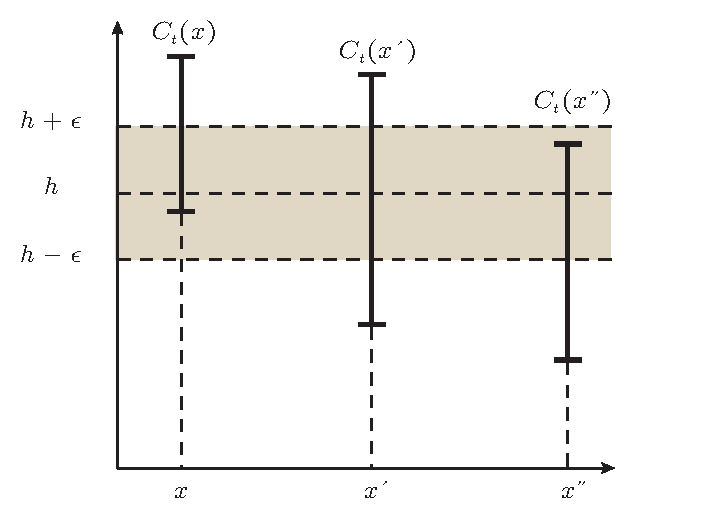
\includegraphics[width=\columnwidth]{figures/class}}
\caption{The three possible configurations of confidence regions.}
\label{fig:class}
\end{center}
\end{figure} 

Initially, all input points are marked as unclassified and the
confidence regions are assigned an infinite range (lines~1--4). Thereafter,
the algorithm iterates until all points have been classified (line 6).

At each iteration, for every unclassified point
(line~10) the respective confidence region and its range are updated
(lines~11--12) and the point is classified into $H_t$ or $L_t$ if either
of two criteria is met (lines~13--19). \figref{fig:class} depicts the
three possible cases in more detail. In the case of point $\*x$,
the lowest estimated function value $\min(C_t(\*x))$ is no less
than $h-\epsilon$, therefore the condition in line~13 holds and $\*x$
is moved to $H_t$. For point $\*x''$, the highest estimated
function value $\max(C_t(\*x''))$ is no more than $h+\epsilon$,
therefore the condition in line~16 holds and $\*x''$ is moved to $L_t$.
However, point $\*x'$ satisfies neither condition and, as a consequence,
remains unclassified.

After the above classification procedure, the point in $U_t$
with the largest associated confidence region range $w_t$ is selected for
evaluation (lines~21--22) and the GP model predictions are updated using the
newly acquired measurement (line 23). Finally, once the iterations have
completed and all points are classified, the estimated sets $\hat{H}$ and
$\hat{L}$ are returned  (lines~26--27).

\begin{algorithm}[tb]
  \caption{The \acl algorithm}
  \label{alg:acl}
\begin{algorithmic}[1]
  \REQUIRE input space $D$, GP prior ($\mu_0$, $\sigma_0$, $k$),\\
           \hspace{1.9em}threshold value $h$, accuracy parameter $\epsilon$
  \ENSURE predicted sets $\hat{H}$, $\hat{L}$
  \LET{$H_0$}{$\varnothing$}
  \LET{$L_0$}{$\varnothing$}
  \LET{$U_0$}{$D$}
  \LET{$C_0(\*x)$}{$\mathbb{R}$, for all $\*x \in D$}
  \LET{$t$}{1}
  \WHILE{$U_{t-1} \neq \varnothing$}
    \LET{$H_t$}{$H_{t-1}$}
    \LET{$L_t$}{$L_{t-1}$}
    \LET{$U_t$}{$U_{t-1}$}
    \FORALL{$\*x \in U_{t-1}$}
      \LET{$C_{t}(\*x)$}{$C_{t-1}(\*x) \cap Q_t(\*x)$}
      \LET{$w_{t}(\*x)$}{$\max(C_{t}(\*x)) - \min(C_{t}(\*x))$}
      \IF{$\min(C_t(\*x)) + \epsilon \geq h$}
        \LET{$U_t$}{$U_t \setminus \{\*x\}$}
        \LET{$H_t$}{$H_t \cup \{\*x\}$}
      \ELSIF{$\max(C_t(\*x)) - \epsilon \leq h$}
        \LET{$U_t$}{$U_t \setminus \{\*x\}$}
        \LET{$L_t$}{$L_t \cup \{\*x\}$}
      \ENDIF
    \ENDFOR
    \LET{$\*x_t$}{$\argmax_{\*x \in U_t}(w_t(\*x))$}
    \LET{$y_t$}{$f(\*x_t) + \nu_t$}
    \STATE Compute $\mu_t(\*x)$ and $\sigma_t(\*x)$ for all $\*x \in U_t$
    \LET{$t$}{$t + 1$}
  \ENDWHILE
  \LET{$\hat{H}$}{$H_{t-1}$}
  \LET{$\hat{L}$}{$L_{t-1}$}
\end{algorithmic}
\end{algorithm}

\subsection{Theoretical Analysis of \acl}
The convergence analysis of \acl is based on the regularity of the GP kernel
quantified by the maximum information gain of $t$ sampled points
\begin{align*}
\gamma_t = \max_{\*y_t}I(\*y_t; \*f_t),
\end{align*}
where $\*y_t = (y_i)_{1\leq i\leq t}$ and
$\*f_t = (f(\*x_i))_{1\leq i\leq t}$.

The quality of a solution $(\hat{H}, \hat{L})$ returned by \acl with
respect to the classification of a single point $\*x \in D$ can be
judged by the misclassification error
\begin{align*}
\ell(\*x) = \twopartdef{\max\{0, f(\*x) - h\}}{\*x\in \hat{L}}{\max\{0, h - f(\*x)\}}{\*x\in \hat{H}}
\end{align*}
The following theorem establishes bounds on the number of \acl iterations
required to achieve a certain classification quality in terms of the
maximum misclassification error.

\begin{theorem}
\label{thm:acl}
For any $\delta \in (0, 1)$ and $\epsilon \geq 0$,
if $\beta_t = 2\log(|D|\pi^2 t^2/(6\delta))$, then \acl terminates after
at most $T$ iterations, where $T$ is the smallest positive integer
satisfying
\begin{align*}
\frac{T}{\beta_T \gamma_T} \geq \frac{C_1}{4\epsilon^2},
\end{align*}
where $C_1 = 8/log(1 + \sigma^{-2})$.

Furthermore, with probability at least $1-\delta$, no point is
misclassified by more than $\epsilon$, that is
\begin{align*}
\Pr\left\{\max_{\*x\in D}\ell(\*x) \leq \epsilon\right\} \geq 1 - \delta.
\end{align*}
\end{theorem}

\theoremref{thm:acl} is proven using
Lemmas~\ref{lem:srin1}--\ref{lem:prob} (see \appref{sect:app_acl}).

%%%--------------------------------------------------------------------------%%%
%%% Batch
%%%--------------------------------------------------------------------------%%%
\section{Batch measurements}
The batch setting is differentiated from the sequential one seen in the
previous section by the
fact that measurements are not evaluated one by one, but rather several
measurements are performed in parallel and feedback is received after
some delay. In general, the available measurements at each iteration
are determined by a function
$\fb : \mathbb{N} \to \mathbb{N}\cup\{0\}$, such that
$\fb[t] \leq t-1$ for all $t \geq 1$. This means that when selecting
the next measurement at iteration $t$, we have access to evaluated
measurements up to timestep $fb[t]$.

\subsection{The \bacl Algorithm}
As in the sequential case, the selection of measurements is guided by
defining confidence regions using the predicted mean and variance of
the GP model. Because the predicted variance does not depend on the
observed values, we can use in place of $Q_t(\*x)$ the following
confidence interval
\begin{align*}
Q_t^b(\*x) = \left[\mu_{\fb[t]}(\*x) \pm \eta_t^{1/2}\sigma_{t-1}(\*x)\right],
\end{align*}
where, again, the scaling parameter $\eta_t$ has to be chosen appropriately.

As before, we intersect successive intervals to obtain the following
monotonically decreasing confidence regions
\begin{align*}
C_t^b(\*x) = C_{t-1}^b(\*x) \cap Q_t^b(\*x)
\end{align*}
with $C_0^b(\*x) = \mathbb{R}$ and range
\begin{align*}
w_t^b(\*x) = \max(C_t^b(\*x)) - \min(C_t^b(\*x)).
\end{align*}

\begin{algorithm}[!t]
  \caption{The \bacl algorithm}
  \label{alg:bacl}
\begin{algorithmic}[1]
  \REQUIRE input space $D$, GP prior ($\mu_0$, $\sigma_0$, $k$),\\
           \hspace{1.9em}threshold value $h$, accuracy parameter $\epsilon$,\\
           \hspace{1.9em}feedback function $\fb$
  \ENSURE predicted sets $\hat{H}$, $\hat{L}$
  \LET{$H_0$}{$\varnothing$}
  \LET{$L_0$}{$\varnothing$}
  \LET{$U_0$}{$D$}
  \LET{$C_0^b(\*x)$}{$\mathbb{R}$, for all $\*x \in D$}
  \LET{$t_{fb}$}{0}
  \LET{$t$}{1}
  \WHILE{$U_{t-1} \neq \varnothing$}
    \LET{$H_t$}{$H_{t-1}$}
    \LET{$L_t$}{$L_{t-1}$}
    \LET{$U_t$}{$U_{t-1}$}
    \FORALL{$\*x \in U_{t-1}$}
      \LET{$C_{t}^{b}(\*x)$}{$C_{t-1}^{b}(\*x) \cap Q_t^{b}(\*x)$}
      \LET{$w_{t}^{b}(\*x)$}{$\max(C_{t}^{b}(\*x)) - \min(C_{t}^{b}(\*x))$}
      \IF{$\min(C_t^{b}(\*x)) + \epsilon \geq h$}
        \LET{$U_t$}{$U_t \setminus \{\*x\}$}
        \LET{$H_t$}{$H_t \cup \{\*x\}$}
      \ELSIF{$\max(C_t^{b}(\*x)) - \epsilon \leq h$}
        \LET{$U_t$}{$U_t \setminus \{\*x\}$}
        \LET{$L_t$}{$L_t \cup \{\*x\}$}
      \ENDIF
    \ENDFOR
    \LET{$\*x_t$}{$\argmax_{\*x \in U_t}(w_t^{b}(\*x))$}
    \IF{$\fb[t+1] > t_{fb}$}
      \FOR{$i = t_{fb}+1,\ldots,t$}
        \LET{$y_i$}{$f(\*x_i) + \nu_i$}
      \ENDFOR
      \STATE Compute $\mu_t(\*x)$ for all $\*x \in U_t$
      \LET{$t_{fb}$}{$t$}
    \ENDIF
    \STATE Compute $\sigma_t(\*x)$ for all $\*x \in U_t$
    \LET{$t$}{$t + 1$}
  \ENDWHILE
  \LET{$\hat{H}$}{$H_{t-1}$}
  \LET{$\hat{L}$}{$L_{t-1}$}
\end{algorithmic}
\end{algorithm}

\algoref{alg:bacl} shows the pseudocode of the \bacl algorithm. The main
difference from the sequential version can be seen in lines~23--30.
In particular, after selecting the point of measurement at iteration $t$
in a similar fashion to the sequential version (line~22), the algorithm
checks whether there is some new feedback available (line~23). If that
is the case, measurements from the latest obtained feedback point ($t_{fb}$)
up to the current iteration are obtained (lines~24--26), the predicted
means are updated (line~27), and the feedback pointer $t_{fb}$
is updated (line~28). Note that the predicted variances are updated at
each iteration (line~30), even if there is no new feedback available.

\subsection{Theoretical Analysis of \bacl}
Compared to the analysis of \acl, the main addition required in the case of
\bacl is to ensure that the new confidence regions $Q_t^b(\*x)$ still
contain $f(\*x)$ with high probability. To that end, a bound on the
conditional mutual information between $f$ and the measurements
obtained during the batch selection, given the already available feedback,
is obtained and used to adjust $\eta_t$.

The following theorem is the analog to \theoremref{thm:acl} for the
\bacl algorithm.

\begin{theorem}
\label{thm:bacl}
Assume that for all $t \geq 1$ the maximum conditional mutual information
acquired by any set of measurements since the last feedback is bounded
by a constant $C \geq 0$, i.e.
\begin{align*}
\max_{A\subseteq D, |A|\leq B-1} I(f; \*y_A \mid \*y_{1:fb[t]}) \leq C
\end{align*}
Then, for any $\delta \in (0, 1)$ and $\epsilon \geq 0$,
if $\eta_t = e^C\beta_{fb[t]+1}$, \bacl terminates after
at most $T$ iterations, where $T$ is the smallest positive integer
satisfying
\begin{align*}
\frac{T}{\eta_T \gamma_T} \geq \frac{C_1}{4\epsilon^2},
\end{align*}
where $C_1 = 8/log(1 + \sigma^{-2})$.

Furthermore, with probability at least $1-\delta$, no point is
misclassified by more than $\epsilon$, that is
\begin{align*}
\Pr\left\{\max_{\*x\in D}\ell(\*x) \leq \epsilon\right\} \geq 1 - \delta.
\end{align*}
\end{theorem}

\theoremref{thm:bacl} is proven using
Lemmas~\ref{lem:cmi}--\ref{lem:batch}  (see \appref{sect:app_bacl}).

\bibliography{acl}
\bibliographystyle{icml2013}


\appendix
%%%--------------------------------------------------------------------------%%%
%%% Appendix sequential
%%%--------------------------------------------------------------------------%%%
\section{Proof of \theoremref{thm:acl}} \label{sect:app_acl}

\begin{lemma}
\label{lem:srin1}
For any $\delta \in (0, 1)$, if $\beta_t = 2\log(|D|\pi_t/\delta)$, where
$\sum_{t\geq1}\pi_t^{-1}$ and $\pi_t > 0$, then the following holds with
probability at least $1-\delta$
\begin{align*}
|f(\*x) - \mu_{t-1}(\*x)| \leq \beta_t^{1/2}\sigma_{t-1}(\*x),\ \forall \*x \in D\ \forall t \geq 1
\end{align*}
In particular, we can choose $\pi_t = \pi^2 t^2/6$.
\end{lemma}
\begin{proof}
See Lemma 5.1 in \cite{srinivas2010}.
\end{proof}

\begin{cor}
\label{cor:cs}
For any $\delta \in (0, 1)$ and $\beta_t$ as above, the following holds
with probability at least $1-\delta$
\begin{align*}
f(\*x) \in C_t(\*x),\ \forall \*x \in D\ \forall t \geq 1
\end{align*}
\end{cor}

\begin{lemma}
\label{lem:wb}
The following holds for any $t \geq 1$
\begin{align*}
w_t(\*x_t) \leq 2\beta_t^{1/2}\sigma_{t-1}(\*x_t)
\end{align*}
\end{lemma}
\begin{proof}
The confidence regions of the selected points are defined as
$C_t(\*x_t) = C_{t-1}(\*x_t) \cap Q_t(\*x_t)$, therefore, by
definition of $w_t(\*x_t)$
\begin{align*}
w_t(\*x_t) &= \max(C_t(\*x_t)) - \min(C_t(\*x_t))\\
&\leq \max(Q_t(\*x_t)) - \min(Q_t(\*x_t))\\
&=2\beta_t^{1/2}\sigma_{t-1}(\*x_t)
\end{align*}
\end{proof}

\begin{lemma}
\label{lem:dec}
When running \acl, $w_t(\*x_t)$ is nonincreasing in $t$.
\end{lemma}
\begin{proof}
From the definition of the confidence regions
$C_t(\*x_t) = C_{t-1}(\*x_t) \cap Q_t(\*x_t)$, it follows that
$w_t(\*x_t) \leq w_{t-1}(\*x_t)$. From the selection rule
$\*x_t = \argmax_{\*x\in U_t}(w_t(\*x))$ and the monotonicity of
$U_t$ ($U_t \supseteq U_{t-1}$), it follows that
$w_{t-1}(\*x_t) \leq w_{t-1}(\*x_{t-1})$.
\end{proof}

\begin{lemma}
\label{lem:ig}
Denoting $\*y_t = (y_i)_{1\leq i\leq t}$ and
$\*f_t = (f(\*x_i))_{1\leq i\leq t}$,
the information gain for the selected points up to iteration $t$ can be
expressed in terms of the predictive variances as follows
\begin{align*}
I(\*y_t; \*f_t) = \frac{1}{2}\sum_{i=1}^t \log(1 + \sigma^{-2}\sigma_{i-1}^2(\*x_i))
\end{align*}
\end{lemma}
\begin{proof}
See Lemma 5.3 in \cite{srinivas2010}.
\end{proof}

\begin{lemma}
When running \acl with $\beta_t$ as in \lemmaref{lem:srin1}, it holds that
\begin{align*}
w_t(\*x_t) \leq \sqrt{\frac{C_1 \beta_t \gamma_t}{t}},\ \forall t \geq 1,
\end{align*}
where $C_1 = 8 / \log(1 + \sigma^{-2})$.
\end{lemma}
\begin{proof}
Similarly to Lemma 5.4 in \cite{srinivas2010},
from \lemmaref{lem:wb} it follows that for any $i \geq 1$
\begin{align*}
w_i^2(\*x_i) &\leq 4\beta_i\sigma_{i-1}^2(\*x_i)\\
&\leq 4\beta_i\sigma^2(\sigma^{-2}\sigma_{i-1}^2(\*x_i))\\
&\leq 4\beta_i\sigma^2 C_2\log(1 + \sigma^{-2}\sigma_{i-1}^2(\*x_i))
\end{align*}
where $C_2 = \sigma^{-2}/\log(1 + \sigma^{-2})$.
Using \lemmaref{lem:ig} in the above expression, the fact that $\beta_i$
is nondecreasing in $i$, and defining $C_1 = 8\sigma^2C_2$,
we get for any $t \geq 1$
\begin{align*}
C_1\beta_t\gamma_t &\geq C_1\beta_t I(\*y_t; \*f_t)\\
                   &\geq \sum_{i=1}^t w_i^2(\*x_i)\\
                   &\geq \frac{1}{t}\left(\sum_{i=1}^t w_i(\*x_i)\right)^2 \tag*{\textrm{(by Cauchy-Schwarz)}}\\
                   &= t \left(\frac{1}{t}\sum_{i=1}^t w_i(\*x_i)\right)^2\\
                   &\geq t w_t^2(\*x_t) \tag*{\textrm{(by \lemmaref{lem:dec})}}
\end{align*}
\end{proof}

\begin{lemma}
When running \acl, if for some $t \geq 1$ $w_t(\*x_t) \leq 2\epsilon$,
then $U_{t+1} = \varnothing$.
\end{lemma}
\begin{proof}
Assume that $U_{t+1} \neq \varnothing$, i.e. there exists a point
$\*x \in U_t$, which does not meet the classification conditions in
lines~13 and 16 of \algoref{alg:acl}. Consequently, that point
satisfies $\max(C_{t+1}(\*x)) > h + \epsilon$ and
$\min(C_{t+1}(\*x)) < h - \epsilon$. It follows that
\begin{align*}
2\epsilon &< \max(C_{t+1}(\*x)) - \min(C_{t+1}(\*x))\\
&= w_{t+1}(\*x) \leq w_t(\*x) \leq w_t(\*x_t)
\end{align*}
The last two inequalities follow from the intersection property of
the confidence regions and the selection rule of $\*x_t$ respectively.
The inequality $2\epsilon < w_t(\*x_t)$ contradicts the assumption, which
proves the lemma.
\end{proof}

\begin{cor}
\label{cor:iter}
The \acl algorithm terminates after at most $T$ iterations, where $T$
is the smallest positive integer satisfying
\begin{align*}
\frac{T}{\beta_T \gamma_T} \geq \frac{C_1}{4\epsilon^2}
\end{align*}
\end{cor}

\begin{lemma}
\label{lem:prob}
For any $\delta \in (0, 1)$, after running \acl with any $\epsilon \geq 0$
and with $\beta_t$ as in \lemmaref{lem:srin1}, with probability at least
$1-\delta$ no point $\*x \in D$ will have been missclassified by more
than $\epsilon$, that is
\begin{align*}
\Pr\left\{\max_{\*x\in D}\ell(\*x) \leq \epsilon\right\} \geq 1 - \delta
\end{align*}
\end{lemma}
\begin{proof}
The lemma follows directly from \corref{cor:cs} and the classification
conditions in lines~13 and 16 of \algoref{alg:acl}.
\end{proof}

\theoremref{thm:acl} follows immediately from \corref{cor:iter}
and \lemmaref{lem:prob}.

%%%--------------------------------------------------------------------------%%%
%%% Appendix batch
%%%--------------------------------------------------------------------------%%%
\section{Proof of \theoremref{thm:bacl}} \label{sect:app_bacl}
\begin{lemma}
\label{lem:cmi}
For any $\*x \in D$ and $t \geq 1$
the ratio of $\sigma_{fb[t]}(\*x)$ to $\sigma_{t-1}(\*x)$ is bounded
as follows
\begin{align*}
\frac{\sigma_{fb[t]}(\*x)}{\sigma_{t-1}(\*x)} \leq \exp\left\{I(f; \*y_{fb[t]+1:t-1} \mid \*y_{1:fb[t]}\right\}
\end{align*}
\end{lemma}
\begin{proof}
See Lemma 1 in \cite{desautels2012}.
\end{proof}

\begin{lemma}
\label{lem:batch}
Assume that for all $t \geq 1$ the maximum conditional mutual information
acquired by any set of measurements since the last feedback is bounded
by a constant $C \geq 0$, i.e.
\begin{align}
\label{eq:cmi}
\max_{A\subseteq D, |A|\leq B-1} I(f; \*y_A \mid \*y_{1:fb[t]}) \leq C
\end{align}
Then, if $\eta_t = e^{2C}\beta_{fb[t]+1}$, the following holds with probability
at least $1 - \delta$
\begin{align*}
f(\*x) \in Q_t^{b}(\*x),\ \forall \*x \in D\ \forall t \geq 1
\end{align*}
\end{lemma}
\begin{proof}
From \lemmaref{lem:cmi} and \eqtref{eq:cmi}, it follows that for any
$\*x \in D$ and $t \geq 1$
\begin{align*}
&\frac{\sigma_{fb[t]}(\*x)}{\sigma_{t-1}(\*x)} \leq \exp\left\{I(f; \*y_{fb[t]+1:t-1} \mid \*y_{1:fb[t]}\right\} \leq e^C\\
\Rightarrow\ & e^C \sigma_{t-1}(\*x) \geq \sigma_{fb[t]}(\*x)
\end{align*}
Using this, the range of $Q_t^{b}(\*x)$ can be related to the range
of $Q_{fb[t]+1}(\*x)$ as follows
\begin{align*}
2\eta_t^{1/2}\sigma_{t-1}(\*x) = 2 e^C \beta_{fb[t]+1}^{1/2}\sigma_{t-1}(\*x) \geq 2\beta_{fb[t]+1}^{1/2}\sigma_{fb[t]}(\*x)
\end{align*}
Furthermore, $Q_t^{b}(\*x)$ and $Q_{fb[t]+1}(\*x)$ have the same midpoint,
namely $\mu_{fb[t]}(\*x)$, therefore the above range inequality implies that
\begin{align}
\label{eq:qbss}
Q_t^{b}(\*x) \supseteq Q_{fb[t]+1}(\*x),\ \forall \*x \in D\ \forall t \geq 1
\end{align}
Finally, from \lemmaref{lem:srin1} we have that
\begin{align*}
&\Pr\{f(\*x) \in Q_{fb[t]+1}(\*x)\} \geq 1 - \delta,\ \forall \*x \in D\ \forall t \geq 1\\
\stackrel{\eqref{eq:qbss}}{\Rightarrow}\ & \Pr\{f(\*x) \in Q_t^{b}(\*x)\} \geq 1 - \delta,\ \forall \*x \in D\ \forall t \geq 1
\end{align*}
\end{proof}

\begin{cor}
\label{cor:batch}
Given the assumptions of \lemmaref{lem:batch}, the following holds with
probability at least $1-\delta$
\begin{align*}
f(\*x) \in C_t^{b}(\*x),\ \forall \*x \in D\ \forall t \geq 1
\end{align*}
\end{cor}

Note that \corref{cor:batch} is completely analogous to \corref{cor:cs}.
Thus, the results of Lemmas~\ref{lem:wb}--\ref{lem:prob} also hold for
the case of \bacl, provided that $\eta_t$, as defined in \lemmaref{lem:batch},
is used in place of $\beta_t$, which proves \theoremref{thm:bacl}.

\end{document} 


% This document was modified from the file originally made available by
% Pat Langley and Andrea Danyluk for ICML-2K. This version was
% created by Lise Getoor and Tobias Scheffer, it was slightly modified  
% from the 2010 version by Thorsten Joachims & Johannes Fuernkranz, 
% slightly modified from the 2009 version by Kiri Wagstaff and 
% Sam Roweis's 2008 version, which is slightly modified from 
% Prasad Tadepalli's 2007 version which is a lightly 
% changed version of the previous year's version by Andrew Moore, 
% which was in turn edited from those of Kristian Kersting and 
% Codrina Lauth. Alex Smola contributed to the algorithmic style files.  
